\chapter{Methods}

While the self-supervised denoising methods discussed so far eliminate the need for clean data, most still require large datasets of noisy images or are limited to specific noise types.
A notable exception is the Deep Image Prior (DIP) introduced by Ulyanov~et al.~\cite{DIP}.
DIP is a zero-shot method, meaning it operates on a single noisy sample, and does not make any explicit assumptions about the noise distribution.

In this chapter, we present DIP and its various extensions.
First, we describe the fundamental principles of DIP, followed by common techniques used to further regularize the solution.
Finally, we explore additional DIP-based approaches that build upon these foundations.

\section{Deep Image Prior}

As discussed in Section~\ref{sec:denoising}, denoising is an ill-posed inverse problem and therefore appropriate regularization is crucial in order to obtain plausible solutions.
This is typically expressed as an optimization problem of the form
\begin{equation}\label{eq:ip-optim}
    \hat{x} = \argmin_x L(x,y) + R(x),
\end{equation}
where $L(x,y)$ is a data fidelity term that ensures that the denoised estimate $\hat{x}$ stays close to the noisy signal $y$ and $R(x)$ is the regularizer.
Most traditional, non-deep-learning methods, such as total variation denoising~\cite{TV}, rely on an explicit regularization term.
The self-supervised methods discussed in Section~\ref{sec:self-supervised} do not necessarily include such a term; however, they do make specific assumptions about the solution (e.g., zero-mean or spatially independent noise), which are implicitly encoded in the training procedure --- through techniques like subsampling or masking.

In contrast, DIP does not make any explicit assumptions about the noise or image structure.
Instead, it relies solely on the architecture of a convolutional neural network to implicitly regularize the solution.
The key idea is to parameterize an image $x$ as the output of an CNN $f_\theta$ through $x = f_\theta(z)$, where $z$ refers to a random vector, e.g., $z \sim \unormal$.
\begin{figure}
    \centering
    \begin{tikzpicture}[scale=1.5]
        \useasboundingbox (-3,3.5) rectangle (3,-0.5);

        % Coords
        \coordinate (t0) at (1,3.5);
        \coordinate (t1) at (-0.2,3.3);
        \coordinate (t2) at (-1.4,2.9);
        \coordinate (t3) at (-2.4,2);
        \coordinate (t4) at (-2.2,0.8);
        \coordinate (t5) at (-1,0.2);
        \coordinate (x) at (-1.8,1.8);
        \coordinate (y) at (0,0);
        \coordinate (p) at (-0.6,0.6);

        % Curves
        \draw[very thick, RoyalBlue, dashed] (x) -- (y);
        \draw[very thick, black, -{Latex[length=8pt,width=8pt]}, shorten >=4pt] plot [smooth, tension=0.7] coordinates {(t0) (t1) (t2) (t3) (t4) (t5) (y)};
        \draw[very thick, JungleGreen, -{Latex[length=8pt,width=8pt]}, shorten >=4pt] (t0) to[out=-80, in=10] (p);
        \draw[very thick, Orchid, -{Latex[length=8pt,width=8pt]}, shorten >=4pt] (t0) .. controls (4,2) and (3,0.5) .. (y);

        % Points
        \fill[black] (t0) circle (2pt);
        \fill[black] (t1) circle (2pt);
        \fill[black] (t2) circle (2pt);
        \fill[Maroon] (t3) circle (2pt);
        \fill[black] (t4) circle (2pt);
        \fill[black] (t5) circle (2pt);
        \fill[RoyalBlue] (x) circle (2pt);
        \fill[RoyalBlue] (y) circle (2pt);

        % Labels
        \node[above, yshift=2pt] at (t0) {$t_0$};
        \node[above, yshift=2pt] at (t1) {$t_1$};
        \node[above, yshift=2pt] at (t2) {$t_2$};
        \node[left, xshift=-2pt, Maroon] at (t3) {$t_3$};
        \node[left, xshift=-2pt] at (t4) {$t_4$};
        \node[below, yshift=-2pt] at (t5) {$t_5$};
        \node[below, yshift=-2pt, RoyalBlue] at (x) {$x$};
        \node[below, yshift=-2pt, RoyalBlue] at (y) {$y$};

        \node[below] at (-0.8, 3) {\sffamily DIP};
        \node[below, JungleGreen, align=center] at (1.7,2) {\sffamily Conventional\\prior};
        \node[below, Orchid] at (2,0.3) {\sffamily No prior};
    \end{tikzpicture}
    \caption{
        The effect of priors.
        Without regularization, the optimization leads directly to the noisy image $y$.
        Conventional priors shift the solution closer to the clean image $x$.
        DIP will eventually overfit to $y$, but often the optimization path will pass close to $x$, with the optimal stopping point marked in red.
        Figure adapted from~\cite{DIP}.
    }\label{fig:priors}
\end{figure}
This means that instead of optimizing $x$ directly, the reconstruction is constrained by the network's ability to map $z$ to a plausible image.
In terms of Equation~(\ref{eq:ip-optim}), the MSE is used as the loss function and the regularizer $R(x)$ is replaced with the implicit prior induced by the network structure, leading to the following optimization:
\begin{equation}
    \theta^* = \argmin_\theta \norm{f_\theta(z) - y}_2^2.
\end{equation}
After training the network using gradient descent, the denoised estimate is then obtained as $\hat{x} = f_{\theta^*}(z)$.
The random vector $z$ remains fixed throughout the training process.
The regularizing effect of this parameterization relies on the observation that CNNs tend to capture structured patterns (e.g., edges and textures) before fitting to high-frequency noise.
However, since the network is sufficiently expressive, it will eventually memorize the noise, leading to overfitting.
Thus, it is crucial to identify the optimal stopping point, at which the network successfully learned the underlying image structure while minimizing the influence of noise.
This process is visualized in Figure~\ref{fig:priors}.
Formally, this regularizer can be expressed as
\begin{equation}
    R(x) = \begin{cases}
        0 &\text{$f_\theta$ can produce $x$ in $N$ steps}\\
        +\infty &\text{else},
    \end{cases}
\end{equation}
where $N$ refers to a fixed maximum number of iterations.
However, such a fixed stopping point is not ideal because the optimal stopping point depends on factors such as the specific image $x$, the random vector $z$ and also the initial network parameters $\theta_0$.

\subsection{Early Stopping}

\begin{figure}[t]
    \centering
    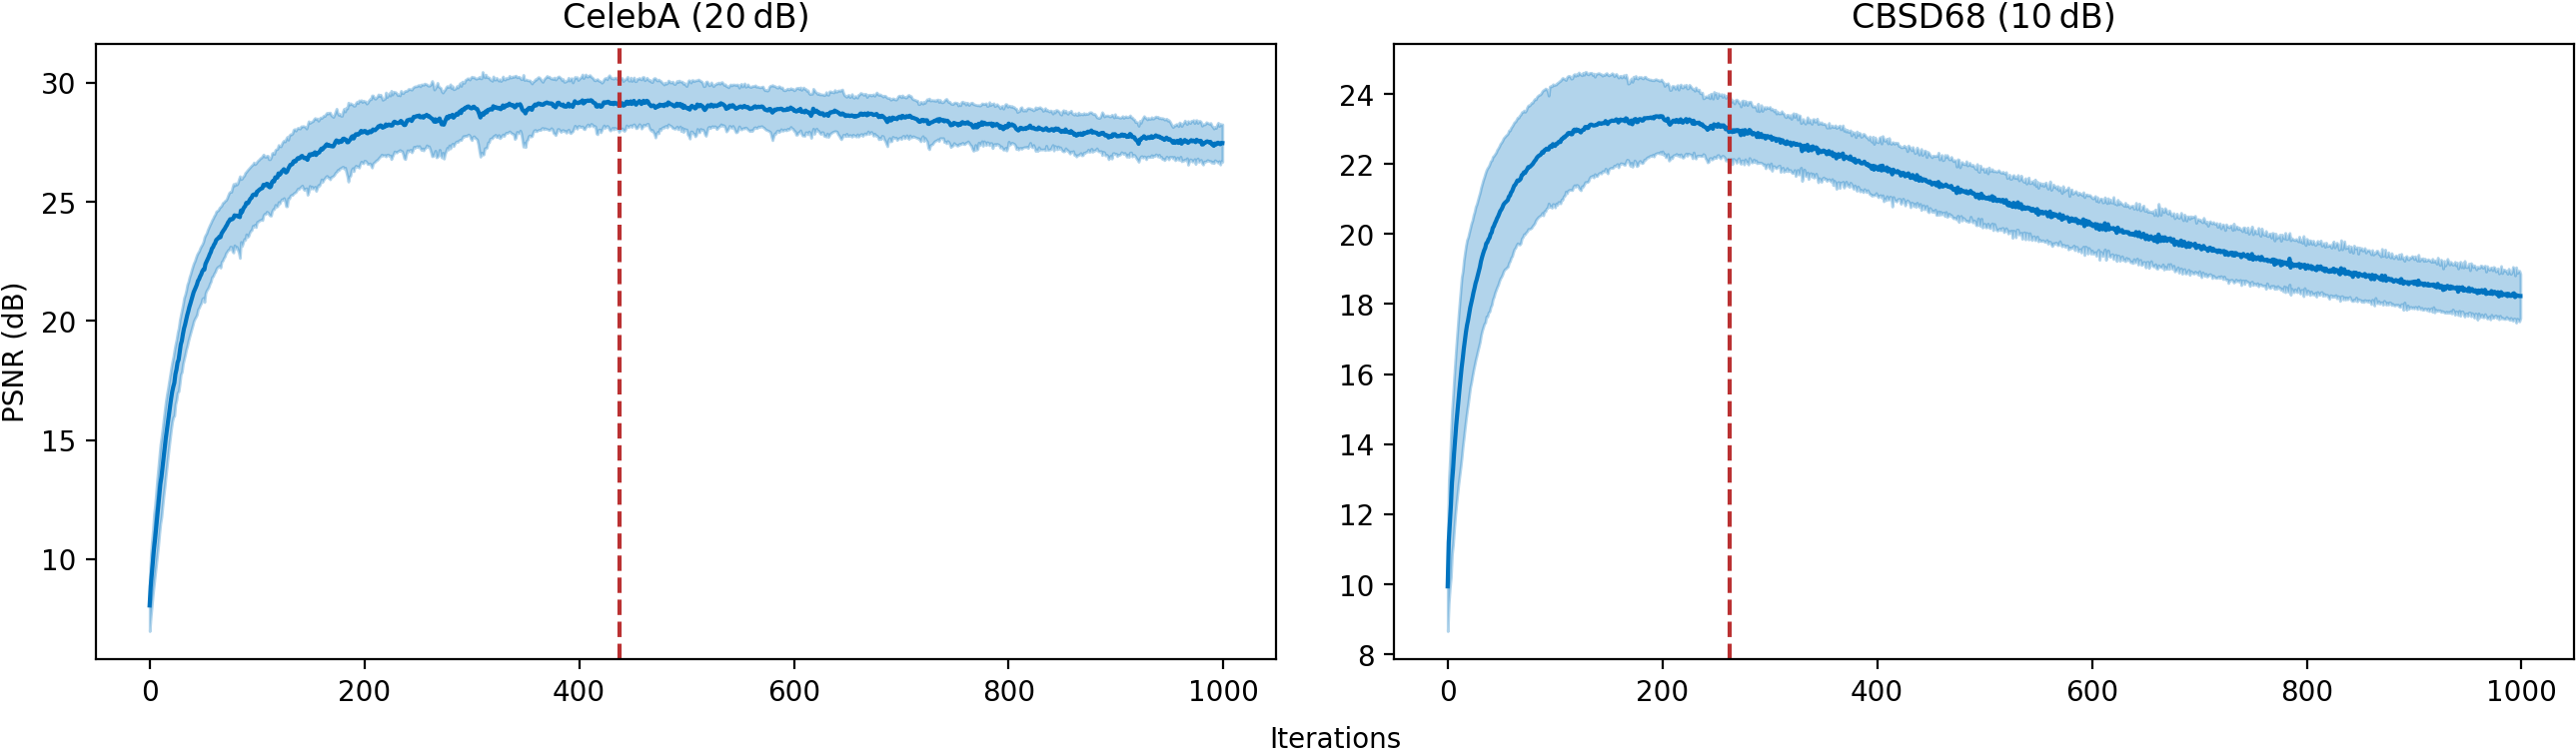
\includegraphics[width=\textwidth]{img/fig_4.2.png}
    \caption{
        Early stopping via windowed moving variance on different datasets and noise levels.
        Image quality is evaluated on 20 random images from the CelebA~\cite{CelebA} (left) and CBSD68~\cite{CBSD68} (right) datasets, with Gaussian noise added at specified PSNR levels.
        The blue line represents the mean PSNR, the light blue shaded area indicates the standard deviation.
        The red line marks the average detected stopping point.
    }\label{fig:early-stopping}
\end{figure}

The process of halting training to mitigate overfitting is known as early stopping (ES).
As discussed earlier, a fixed stopping point generally does not work well, so we need to find a way to dynamically detect optimal stopping points during training.
If the clean ground-truth image $x$ were available, one could simply track image quality using an appropriate metric, e.g., PSNR or SSIM, and stop training at its peak.
However, since $x$ is inherently unknown in the denoising setting, we need an alternative criterion to determine when to stop.
Some image quality metrics do not require a clean reference~\cite{BRISQUE}, but they are not very effective for early stopping.

Wang et al.~\cite{ES} instead propose a criterion based on the running variance of the DIP reconstructions over time.
Let $\{x_t\}_{t \geq 1}$ denote the sequence of the respective denoised estimates $x_t = f_{\theta_t}(z)$ at iteration $t$.
The authors observe that the MSE $\norm{x_t-x}_F^2$ initially drops as the networks learns the image structure, and then rises again due to overfitting to noise, leading to a U-shaped curve.
The challenge remains to detect the minimum of said curve without access to $x$.
To achieve this, they consider the running variance over a window of $W$ iterations, given by
\begin{equation}\label{eq:Var}
    \Var(t) = \frac{1}{W} \sum_{w=0}^{W-1} \norm[\bigg]{x_{t+w}-\frac{1}{W} \sum_{i=0}^{W-1} x_{t+i}}_F^2.
\end{equation}
Intuitively, when $t$ is near the optimal stopping point, $x_t$ should be close to $x$, leading to $\frac{1}{W} \sum_{w=0}^{W} x_t \approx x$.
Plugging this back into Equation~(\ref{eq:Var}), we see that when $t$ is near the optimum, $\Var(t)$ approximates the average MSE across the window.
Therefore, they propose using the variance curve's minimum as the stopping point.
To improve robustness, a patience parameter $P$ allows the variance to stagnate for up to $P$ iterations before stopping.
This approach, termed early stopping via windowed moving variance (ES-WMV), is effective across different noise levels and types of images, as demonstrated in Figure~\ref{fig:early-stopping}. 

\subsection{Total Variation}

Another way to prevent overfitting is to incorporate an additional explicit regularization term, such as total variation (TV)~\cite{TV}.
TV encourages piecewise smoothness by penalizing abrupt intensity changes in the image.
Formally, for an image $x \in \R^{W \times H}$, it is defined as
\begin{equation}
    \text{TV}(x) = \frac{1}{W \cdot H} \sum_{i=1}^{W-1} \sum_{j=1}^{H-1} (|x_{i+1,j} - x_{i,j}| + |x_{i,j+1} - x_{i,j}|).
\end{equation}
Liu et al.\ propose combining the implicit network regularization of DIP with an explicit TV regularizer, leading to the method known as DIP-TV~\cite{DIP-TV}.
This results in the following optimization problem:
\begin{equation}
    \theta^* = \argmin_\theta \norm{f_\theta(z) - y}_2^2 + \lambda \text{TV}(f_\theta(z)),
\end{equation}
where $\lambda$ is a hyperparameter controlling the strength of the TV regularization.

\section{Deep Diffusion Image Prior}

% XXX figure: forward/reverse process (see DDPM)

Diffusion models~\cite{Diffusion} have emerged as a powerful class of generative models, achieving state-of-the-art performance in various applications, including image synthesis~\cite{LDM} and solving inverse problems~\cite{DDRM}.
The key idea is to transform complex data distributions into simple ones (such as Gaussian noise) via a forward stochastic process and then train a model to approximate the reverse process.
Formally, given data $x_0 \sim q(x_0)$, the forward diffusion process produces a sequence of increasingly noisy samples $x_t$ over time $t \in [0,T]$ using a fixed Markovian process:
\begin{equation}
    q(x_t \mid x_{t-1}) = \fnormal{x_t}{\sqrt{1 - \beta_t} x_{t-1}}{\beta_t \mathbf{I}},
\end{equation}
where $\beta_t$ is a predefined variance schedule controlling how much noise is added at each step. For sufficiently large $T$, $x_T$ approximates pure Gaussian noise.
A key property of this process is that it admits a closed-form solution at arbitrary timesteps:
\begin{equation}
    q(x_t \mid x_0) = \fnormal{x_t}{\sqrt{\bar{\alpha}_t} x_0}{(1-\bar{\alpha}_t) \mathbf{I}},
\end{equation}
where $\bar{\alpha}_t = \prod_{s=1}^{t} (1 - \beta_s)$ is the cumulative noise factor.
Using the reparameterization trick~\cite{VAE}, this can be expressed as
\begin{equation}
    x_t = \sqrt{\bar{\alpha}_t}x_0 + \sqrt{1-\bar{\alpha}_t}\epsilon, \quad \epsilon \sim \unormal.
\end{equation}
In DDPMs~\cite{DDPM}, a simple linear schedule for $\beta_t$ is used. Nichol et al.~\cite{IDDPM} propose an improved cosine noise schedule, which better balances noise levels across timesteps and leads to higher sample quality.
The goal of the diffusion model is to learn the reverse process, parameterized by a neural network, which iteratively removes noise:
\begin{equation}
    p_\theta(x_{t-1} \mid x_t) = \fnormal{x_{t-1}}{\mu_\theta(x_t, t)}{\beta_t \mathbf{I}},
\end{equation}
where $\mu_\theta$ is a neural network predicting the mean of the denoised sample.
\newpage
Chung et al.\ combine DIP with ideas from diffusion models, leading to the Deep Diffusion Image Prior (DDIP)~\cite{DDIP}.
They observe that both DIP and diffusion models aim to recover a posterior mean:
DIP estimates $\E{x | z,y}$ and diffusion models estimate $\E{x_0 | x_t,y}$.
As both $z$ and $x_t$ are distributed according to $\unormal$ for $t=T$, they propose a generalization of DIP to multiple noise scales. Instead of optimizing from pure noise, they iteratively reduce the noise in $z$, gradually steering it toward the clean image $x_0$.
\begin{align}
    \text{for}\ t=T,\dots,1:\ &\theta_{t-1} = \argmin_{\theta_t} \norm{f_{\theta_t}(x_t) - y}_2^2,\\
    &x_{t-1} = \sqrt{\bar{\alpha}_t}f_{\theta_{t-1}}(x_t) + \sqrt{1-\bar{\alpha}_t}\epsilon, \quad \epsilon \sim \unormal.
\end{align}
In practice, DDIP uses a pre-trained diffusion model as $f_\theta$ and adapts the underlying prior distribution using LoRA~\cite{LoRA} --- optimizing only a small set of additional parameters.
However, since this work focuses strictly on zero-shot methods, we consider using a completely untrained network, as $f_\theta(x_t)$ can still be seen as an estimate of $x_0$ after a sufficient number of initial iterations.
Furthermore, we use a modified cosine schedule: 
\begin{equation}
    \bar{\alpha}_t = 0.8\cos\left(\frac{t}{T}\cdot\frac{\pi}{2}\right)^2+0.1.
\end{equation}

\section{Self-Guided Deep Image Prior}\label{sec:SG-DIP}

Another extension of DIP is the Self-Guided Deep Image Prior (SG-DIP)~\cite{SG-DIP}.
Similar to DDIP, it also iteratively updates the network input; however, instead of doing so explicitly, it achieves this implicitly by optimizing both the network's parameters and the input itself.
Formally, the proposed training objective is defined as:
\begin{equation}\label{eq:SG-DIP}
    \theta^*,z^* = \argmin_{\theta, z} \norm{\E[n]{f_\theta(z + n)} - y}_2^2 + \lambda\norm{\E[n]{f_\theta(z + n)} - z}_2^2,
\end{equation}
where $y$ refers to the noisy image, $z$ is a random tensor, $n$ is Gaussian noise sampled as $n \sim \normal$ and $\lambda$ is a hyperparameter balancing the two terms.
Empirically, the authors find that setting $\sigma = \frac{\max(z)}{2}$ yields good results.
The first term enforces data fidelity, while the second term acts as a regularization term, encouraging the network to behave as a denoiser by constraining the output to be close to the learned input $z$, thereby mitigating overfitting. 
The expectation over the noise distribution helps to stabilize the learned mapping; the denoised estimate is then obtained as $\hat{x} = \E[n]{f_\theta(z + n)}$.
In practice, the expectation is approximated by averaging the outputs of $k$ different noise samples.

This objective naturally induces a structured learning process:
Ideally, the network first learns to capture the general structure of the image.
Due to the optimization of $z$ and the regularization term, both the input and output should provide a reasonable estimate of the clean image.
At this stage, vanilla DIP would typically begin to overfit.
However, in SG-DIP, the regularization term constrains the output from deviating too much from the input, making it costly for the network to fit the noise.  % XXX layout --- since doing so would introduce global alterations to the output.

\begin{figure}
    \centering
    \begin{tikzpicture}[scale=1]
        \node[anchor=south west,inner sep=0,label=above:{$z$}] (z) at (0,0) {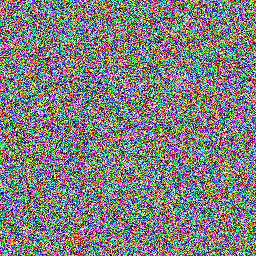
\includegraphics[width=2cm]{img/fig_4.3_z.png}};
        \node[anchor=south west,draw,fill=gray!10,rounded corners,minimum height=2cm,minimum width=1cm] (f) at (3,0) {$f_\theta$};
        \node[anchor=south west,inner sep=0,label=above:{$\hat{x}$}] (x) at (5,0) {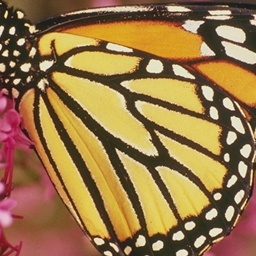
\includegraphics[width=2cm]{img/fig_4.3_x.png}};
        \node[anchor=south west,inner sep=0,label=above:{$y$}] (y) at (8,0) {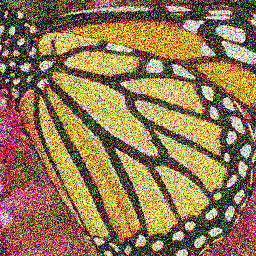
\includegraphics[width=2cm]{img/fig_4.3_y.png}};
        \node[anchor=south west,draw,fill=gray!10,rounded corners,minimum width=2cm,minimum height=0.7cm] (e) at (0,3) {\tiny $n \sim \normal$};
        \node[anchor=north west,draw,fill=gray!10,rounded corners,minimum width=2cm,minimum height=0.7cm] (s) at (0,-1) {\tiny $\lambda = s(t)$};
        \node[anchor=north west,draw,thick,rounded corners,minimum width=1.5cm,minimum height=0.7cm] (l2) at (3,-1) {$R$};
        \node[anchor=north east,draw,thick,rounded corners,minimum width=1.5cm,minimum height=0.7cm] (l1) at (7,-1) {$L$};

        \draw (z.east) -- (f.west);
        \draw[->] (e.east) to[out=0, in=180] (f.west);
        \draw[->] (f.east) -- (x.west);
        \draw[->] (s.east) -- (l2.west);
        \draw[->] (z.south) to[out=-90, in=90] (l2.north);
        \draw (x.south) to[out=-90, in=90] (l2.north);
        \draw[->] (x.south) to[out=-90, in=90] (l1.north);
        \draw (y.south) to[out=-90, in=90] (l1.north);

    \end{tikzpicture}
    \caption{
        Overview of our adapted SGR-DIP training objective.
        The network input is the sum of $z$ (which is pure noise in the first iteration) and noise sampled from a Gaussian distribution.
        The overall loss consists of two terms: a data fidelity term $L$ and a regularization term $R$.
        $L$ measures the difference between the network output and the noisy image, $R$ ensures that the output stays close to the input.
        The influence of $R$ increases over time through a schedule $s(t)$.
    }\label{fig:SGR-DIP}
\end{figure}

\begin{wrapfigure}{r}{0.48\textwidth}
    \begin{algorithm}[H]
        \caption{SGR-DIP}\label{alg:SGR-DIP}
        \KwIn{noisy image $y$, randomly initialized $z_0$ and $\theta_0$}
        \KwOut{denoised image $\hat{x}$}
        \For{$t=0$ \KwTo $T$}{
            $\hat{x} \gets \mathbf{0}$\\
            \For{$i=0$ \KwTo $k$}{
                sample $n \sim \normal$\\
                $\hat{x} \gets \hat{x} + \frac{1}{k}f_{\theta_t}(z_t+n)$\\
            }
            $\lambda \gets s(t)$\\
            obtain $\theta_{t+1}$ and $z_{t+1}$ via Eq.~\ref{eq:SG-DIP}\\
        }
        \Return $\hat{x}$
    \end{algorithm}
\end{wrapfigure}

Instead, the network is encouraged to refine the output while staying close to the input, effectively suppressing noise without overfitting.
To explicitly reinforce this behavior, we propose gradually increasing $\lambda$ throughout training according to a schedule $\lambda = s(t)$, where $t$ denotes the current iteration.
This approach intuitively divides the optimization process into two phases:
Initially, both terms in the objective are balanced, allowing the network to extract the general structure of the image. As training progresses and $\lambda$ increases, the regularization term dominates, restricting the model to only minor refinements.
Therefore, we term this modification Self-Guided Refinement Deep Image Prior (SGR-DIP).
The overall training objective is illustrated in Figure~\ref{fig:SGR-DIP} and Algorithm~\ref{alg:SGR-DIP}.

We observe that the addition of the schedule improves denoising performance; however, we note that the effectiveness of this approach is highly dependent on the specific configuration of the schedule implemented, especially on DAS data.
If the regularization term remains too small for an extended period, there is still a risk of overfitting.
Conversely, if it increases too prematurely, it may hinder further learning before the image structure has been adequately captured.

To address this issue, we also consider a variant in which we replace the random initialization of $z$ with the noisy image $y$.
Note that the two loss terms are still different, as $z$ is optimized throughout training, while $y$ stays constant.
This modification facilitates the network's ability to learn the primary structure of the image. 
However, we observe that it necessitates an increase in the variance of the noise added to $z$ to prevent the network from merely learning the identity function.